%%%%%%%%%%%%%%%%%%%%%%%%%%%%%%%%%%%%%%%%%%%%%%%%%%%%%%%%%%%%%%%%%%%%%%%%%%%%%%%%%
%
% This is a very basic template for mathematical presentations using LaTeX and beamer, aimed at University of Edinburgh students on the Honours Analysis course 2017-2018, for their "Skills" presentations.
%
% This template is just to get you started and to see what the possibilities are.  There is no required format, and you are free to use, discard, edit as much as you like.  I've put in some mathematical content to demonstrate the very basics of LaTeX.  Clearly, you will need to change this.
%
% Except for a few structural comments, I don't comment on the LaTeX itself.  If you have used it before, most of what you know should apply as usual.  If you have not, have a look at the source code, the output, and experiment with editing the code and see what happens.  Most LaTeX code is pretty intuitive, e.g. the command to produce an alpha is \alpha, the command for an integral sign is \int, etc.  You can learn an awful lot by guesswork, trial and error, and google.  
%
% The percent signs "%" are comment signs, and instruct LaTeX to ignore everything following the sign on the same line.  They can be used to comment on the code.
%
%%%%%%%%%%%%%%%%%%%%%%%%%%%%%%%%%%%%%%%%%%%%%%%%%%%%%%%%%%%%%%%%%%%%%%%%%%%%%%%%
%
% The following lines are the preamble.  They help LaTeX set-up the document, but do not print anything yet.



\documentclass{beamer}		% This tells LaTeX the document will be a "beamer" presentation

\mode<presentation>
{
  \usetheme{Madrid}      % or try Darmstadt, Madrid, Warsaw, ...
  \usecolortheme{default} % or try albatross, beaver, crane, ...
  \usefonttheme{serif}  % or try serif, structurebold, ...
  \setbeamertemplate{navigation symbols}{}
  \setbeamertemplate{caption}[numbered]
} 

\usepackage{amsmath}
\usepackage{amssymb}
\usepackage{amsfonts}
\usepackage{bm}
\usepackage{graphicx}

\newcommand{\dd}{\mathrm{d}}

\title[The Multivariate Hawkes Process in High Dimensions:Beyond Mutual Excitation]{The Multivariate Hawkes Process in High Dimensions:Beyond Mutual Excitation}	% Insert your title.  Depending on the theme you choose above, a "short title" might be useful, as it will appear on the footer of each slide.

\author[Shen Yuan]{Shizhe Chen, Ali Shojaie, Eric Shea-Brown, and Daniela Witten} % Insert your name

% \institute[UoE]{University of Edinburgh} % Self-explanatory

\begin{document} 	% Let's begin

% Presentations come in slide frames.  You have to tell LaTeX when to start a frame, and when to end the frame.  The most common error beginners make with beamer is forgetting the \end{frame} command.	

\newcommand{\light}[1]{\textcolor{gray}{#1}}

\begin{frame}	

\titlepage	% Prints a title page populated with the information given in the preamble
	
\end{frame}	




\begin{frame}[noframenumbering]

\begin{itemize}

    \begin{LARGE}
    
    \item Introduction
    
    \item \light{A Brief Overview of the Hawkes Process}
    
    \item \light{A New Approach for Analyzing the Hawkes Process}
    
    \item \light{Application: Cross-Covariance Analysis of the Hawkes Process}

    \end{LARGE}
    
\end{itemize}
	
\end{frame}






\begin{frame}{Challenge}

Previous theoretical work on the Hawkes process is limited to a special case in which a past event can only increase the occurrence of future events, and the link function is linear. However, in neuronal networks and other real-world applications, inhibitory relationships may be present, and the link function may be non-linear.
    
\end{frame}







\begin{frame}{Contributions}

\begin{itemize}
    
    \item Employ a thinning process representation and a coupling construction to bound the dependence coefficient of the Hawkes process.
    
    \item Establish a concentration inequality for second-order statistics of the Hawkes process.
    
    \item Apply this concentration inequality to cross-covariance analysis in the high-dimensional regime and verify the theoretical claims with simulation studies
    
\end{itemize}
    
\end{frame}







\begin{frame}[noframenumbering]

\begin{itemize}

    \begin{LARGE}
    
    \item \light{Introduction}
    
    \item A Brief Overview of the Hawkes Process
    
    \item \light{A New Approach for Analyzing the Hawkes Process}
    
    \item \light{Application: Cross-Covariance Analysis of the Hawkes Process}

    \end{LARGE}
    
\end{itemize}
	
\end{frame}






\begin{frame}{A Brief Overview of the Hawkes Process}

\begin{align}
\lambda_j(t) = \phi_j \left\{\mu_j + \sum_{k=1}^p (\omega_{k,j} * \dd N_k)(t) \right\},\ j=1,\ldots,p,
\end{align}

where

\begin{align*}
(\omega_{k,j} * \dd N_k)(t) = \int_0^\infty \omega_{k,j}(\Delta)\dd N_k(t-\Delta) = \sum_{i:t_{k,i}\leq t} \omega_{k,j}(t-t_{k,i})
\end{align*}

\textbf{Assumption 1} We assume that $\phi_j(\cdot)$ is $\alpha_j-Lipschitz$ for $j=1,\ldots,p$. Let $\Omega$ be a $p \times p$ matrix whose entries are $\Omega_{j,k} = \alpha_j \int_0^\infty |\omega_{k,j}(\Delta)| \dd \Delta$ for $1 \leq j, k \leq p$. We assume that there exists a generic constant $\gamma_\Omega$ such that $\Gamma_{\max}(\Omega) \leq \gamma_\Omega < 1$.

\end{frame}







\begin{frame}{A Brief Overview of the Hawkes Process}

Define the mean intensity as:
\begin{align}
\Lambda_j = \mathbb{E}[\dd N_j(t)]/\dd t, j = 1, \ldots, p.
\end{align}

~\\
Define the (infinitesimal) cross-covariance $\bm{V}(\cdot) = (V_{k,j}(\cdot))_{p \times p}:\mathbb{R} \mapsto \mathbb{R}^{p \times p} $ as:
\begin{align}
V_{k,j}(\Delta) \equiv 
    \begin{cases} 
    \mathbb{E}[\dd N_j(t)\dd N_k(t-\Delta)]/{\dd t \dd (t-\Delta)}-\Lambda_j \Lambda_k,  & j \ne k,  \\
    \mathbb{E}[\dd N_k(t)\dd N_k(t-\Delta)]/{\dd t \dd (t-\Delta)}-\Lambda_k^2-\Lambda_k \delta(\Delta),  & j = k
    \end{cases}
\end{align}
where $\delta(\cdot)$ is the Dirac delta function.

\end{frame}






\begin{frame}[noframenumbering]

\begin{itemize}

    \begin{LARGE}
    
    \item \light{Introduction}
    
    \item \light{A Brief Overview of the Hawkes Process}
    
    \item A New Approach for Analyzing the Hawkes Process
    
    \item \light{Application: Cross-Covariance Analysis of the Hawkes Process}

    \end{LARGE}
    
\end{itemize}
	
\end{frame}






\begin{frame}{Temporal Dependence}
The key idea is to represent the generalized Hawkes process using the thinning process representation to simulate data from the Hawkes process.

\begin{align}
\bar{y}_{k,j} \equiv \frac{1}{T} \int_0^T \int_0^T f(t-t') \dd N_k(t) \dd N_j(t'), 1 \leq j, k \leq p
\end{align}

\begin{align}
y_{k,j,i} \equiv \frac{1}{2\epsilon} \int_{2\epsilon(i-1)}^{2\epsilon i} \int_0^T f(t-t') \dd N_k(t) \dd N_j(t'),
\end{align}

where $f(\cdot)$ is a known function with properties to be specified later, $\epsilon$ is some small constant. $\bar{y}_{k,j}$ can be seen as the average of the sequence $\left\{y_{k,j,i} \right\}_{i=1}^{T/(2\epsilon)}$.
    
\end{frame}









\begin{frame}{Temporal Dependence}
Use the $\tau$-dependence coefficient as a measure of dependence for $\left\{y_{k,j,i} \right\}_{i=1}^{T/(2\epsilon)}$.
\begin{align}
\tau(\mathcal{M}, X) \equiv \mathbb{E}\left[\sup_h \left\{\left| \int h(x)\mathbb{P}_{X|\mathcal{M}}(\dd x) - \int h(x)\mathbb{P}_X (\dd x) \right| \right\} \right]
\end{align}

where $h(\cdot)$ is 1-Lipschitz function, $X$ is a random variable, and $\mathcal{M}$ is $\sigma$-field. For a sequence $\left\{y_{k,j,i} \right\}_{i=1}^{T/(2\epsilon)}$, the temporal dependence is defined as

\begin{align}
\tau_y(l) \equiv \sup_{u \in \left\{1,2,\ldots \right\}} \tau(\mathcal{H}_u^y, y_{k,j,u+l}),
\end{align}

where $l$ is any positive integer, $\mathcal{H}_u^y$ is the $\sigma$-field determined by $\left\{y_{k,j,i} \right\}_{i=1}^{T/(2\epsilon)}$.
    
\end{frame}









\begin{frame}{Temporal Dependence}
\textbf{Lemma 1} Let $X$ be an integrable random variable and $\mathcal{M}$ a $\sigma$-field defined on the same probability space. If the random variable $Y$ has the same distribution as $X$, and is independent of $\mathcal{M}$, then

\begin{align}
\tau(\mathcal{M}, X) \leq \mathbb{E}|X - Y|.
\end{align}

Then, we can get

\begin{align}
\tau_y(l) \leq \sup_u \mathbb{E}\left| \tilde{y}_{k,j,u+l}^u - y_{k,j,u+l} \right|
\end{align}

where $\left\{\tilde{y}_{k,j,i} \right\}_{i=1}^{T/(2\epsilon)}$ is a sequence satisfying the conditions of Lemma 1.

\end{frame}











\begin{frame}{Coupling Process Construction using Thinning}
Let $N_j^{(0)}$, for $j = 1, \ldots, p$, be a homogeneous Poisson process on $\mathbb{R}^2$ with intensity 1. For $n=1$, we construct a p-variate process $\bm{N}^{(1)}$ as

\begin{align}
\dd N_j^{(1)}(t) = N_j^{(0)}([0,\mu_j] \times \dd t), j=1,\ldots,p
\end{align}

where $N_j^{(0)}([0,\mu_j] \times \dd t)$ is the number of points for $N_j^{(0)}$ in the area $[0,\mu_j] \times [t, t+\dd t)$ . For $n \ge 2$, we construct $\bm{N}^{(n)}$ as

\begin{align}
\lambda_j^{(n)}(t) &= \phi_j \left\{\mu_j + (\bm{\omega}_{\cdot,j} * \dd \bm{N}^{(n-1)})(t) \right\}\\
\dd N_j^{(n)}(t) &= N_j^{(0)}([0,\lambda_j^{(n)}(t)] \times \dd t), j=1,\ldots,p.
\end{align}

\end{frame}









\begin{frame}{Coupling Process Construction using Thinning}
Let $\tilde{N}_j^{(0)}$, for $j = 1, \ldots, p$, also be a homogeneous Poisson process on $\mathbb{R}^2$ with intensity 1, but independent of $N_j^{(0)}$. For $n=1$, we construct a p-variate process $\tilde{\bm{N}}^{(1)}$ as

\begin{align}
\dd \tilde{N}_j^{(1)}(t) = 
    \begin{cases}
    \tilde{N}_j^{(0)}([0,\mu_j] \times \dd t), & t \leq z,\\
    N_j^{(0)}([0,\mu_j] \times \dd t), & t > z
    \end{cases}
\end{align}

where $z \equiv 2 \epsilon u$. For $n \ge 2$, we construct $\tilde{\bm{N}}^{(n)}$ as

\begin{align}
\tilde{\lambda}_j^{(n)}(t) &= \phi_j \left\{\mu_j + (\bm{\omega}_{\cdot,j} * \dd \tilde{\bm{N}}^{(n-1)})(t) \right\}\\
\dd \tilde{N}_j^{(n)}(t) &= 
    \begin{cases}
    \dd \tilde{N}_j^{(0)}([0,\tilde{\lambda}_j^{(n)}(t)] \times \dd t), & t \leq z,\\
    \dd N_j^{(0)}([0,\tilde{\lambda}_j^{(n)}(t)] \times \dd t), & t > z
    \end{cases}
\end{align}

\end{frame}










\begin{frame}{Deviation}
\textbf{Theorem 1} Let $N$ be a Hawkes process with intensity of the form (1) satisfying Assumption 1. For any given $z > 0$, there exists a point process $\tilde{\bm{N}}$ satisfying the Lemma 1, called the coupling process of $\bm{N}$. Let $b$ be a constant and define a matrix $\bm{\eta}(b) = (\eta_{j,k}(b))_{p \times p}$ with $\eta_{j,k}(b) = [\alpha_j \int_b^\infty |\omega_{k,j}(\Delta)| \dd \Delta]$. Then, for any $u \ge 0$,

\begin{align}
\mathbb{E} \left|\dd \bm{\tilde{N}}(z+u) - \dd N(z+u)\right| /\dd u \preceq 2v_1 \left\{\bm{\omega}^{\lfloor u/b+1 \rfloor}\bm{J} + \sum_{i=1}^{\lfloor u/b+1 \rfloor} \bm{\Omega}^{i-1} \bm{\eta}(b) \bm{J}  \right\}
\end{align}


\end{frame}







\begin{frame}{Deviation}


\begin{align}
\begin{split}
&\mathbb{E} \left|\dd \bm{\tilde{N}}(t') \dd \bm{\tilde{N}}(z+u) - \dd N(t') \dd N(z+u)\right| / (\dd u \dd t') \\
&\preceq 2v_2 \left\{\bm{\omega}^{\lfloor u/b+2 \rfloor}\bm{J} + \sum_{i=1}^{\lfloor u/b+1 \rfloor} \bm{\Omega}^{i} \bm{\eta}(b) \right\} \bm{J}\bm{J}^T \\
&+ 2v_1^2 \left\{ \bm{J}\bm{J}^T(\bm{\Omega^{\lfloor u/b+1 \rfloor}})^T + \sum_{i=1}^{\lfloor u/b+1 \rfloor} \bm{\eta}(b)\bm{J}\bm{J}^T(\bm{\Omega^i})^T \right\}
\end{split}
\end{align}
where $\preceq$ denotes element-wise inequality, and $v_1$ and $v_2$ are parameters that depend on $\bm{\Lambda, V}$.

\end{frame}










\begin{frame}{Main Result}

\textbf{Assumption 2} There exists a constant $b_0$ such that, for $b \ge b_0$ and some $r > 0$,

\begin{align*}
\max_j \sum_{k=1}^p \int_b^\infty |\omega_{k,j}(\Delta)| \dd \Delta \leq c_1 \exp (-c_2 b^r).
\end{align*}

~\\
\textbf{Assumption 3} For all $j = 1, \ldots, p$, there exists a positive constant $\rho_{\Omega} < 1$ such that $\bm{\Omega}$ satisfies $\sum_{k=1}^p \Omega_{j,k} \leq \rho_{\Omega}$

% \begin{align}
% \Lambda_j = \mu_j + \bm{\Omega}_{j,\cdot} \cdot \left[\sum_{i=1}^\infty \bm{\Omega}^{i-1} \bm{\mu}  \right] = \mu_j + \bm{\Omega}_{j,\cdot} \cdot \bm{\Lambda} \leq mu_j + \rho_\Omega \max_k(\Lambda_k)
% \end{align}

\end{frame}








\begin{frame}{Main Result}

\textbf{Theorem 2} Suppose that $\bm{N}$ is a Hawkes process with intensity (1), which satisfies Assumptions 1–4. Suppose also that the function $f(\cdot)$ has bounded support and $ \max_x |f(x)| \leq C_f$. For any positive integer $l$, the $\tau$-dependence coefficient of $\left\{y_{j,k,i} \right\}_i $ introduced in (7) satisfies 

\begin{align}
\tau_y(l) \leq a_5 \exp(-a_6 l^{r/(r+l)} )
\end{align}

where $r$ is introduced in Assumption 2, and $a_5$ and $a_6$ are parameters that do not depend on $p$ and $T$.

\end{frame}









\begin{frame}{Main Result}

\textbf{Assumption 4} Assume that one of the following two conditions holds.
\begin{itemize}
    \item For all $j=1,\ldots, p$, the link functions $\phi_j(\cdot)$ in (1) are upper-bounded by a positive constant $\phi_{\max}$.
    \item In Assumption 2, the constant $c_1 = 0$.
\end{itemize}

~\\
\textbf{Lemma 2} Suppose $\bm{N}$ is a Hawkes process with intensity (1), which satisfies Assumptions 1 and 4. For any bounded interval $A$, it holds that, for $j=1,\ldots,p$, $P(N_j(A)>n) \leq \exp (1-n/K)$ for some constant $K$.


\end{frame}






\begin{frame}{Main Result}

\textbf{Theorem 3} Suppose that $\bm{N}$ is a Hawkes process with intensity (1), which satisfies Assumptions 1–4. Suppose also that the function $f(\cdot)$ has bounded support and $\max_x |f(x)| \leq C_f$. Then, for $1 \leq j \leq k \leq p$,

\begin{align}
\begin{split}
&\mathbb{P}\left(\bigcap_{1 \leq j \leq k \leq p}[|\bar{y}_{k,j} -\mathbb{E}\bar{y}_{k,j}| \ge c_3 T^{-(2r+1)/(5r+2)}]  \right) \\
&\leq c_4 p^2 T \exp \left(-c_5 T^{r/(5r+2)} \right),
\end{split}
\end{align}

where $r$ is introduced in Assumption 2, and $c_3$, $c_4$ and $c_5$ are parameters that do not depend on $p$ and $T$.

\end{frame}







\begin{frame}[noframenumbering]

\begin{itemize}

    \begin{LARGE}
    
    \item \light{Introduction}
    
    \item \light{A Brief Overview of the Hawkes Process}
    
    \item \light{A New Approach for Analyzing the Hawkes Process}
    
    \item Application: Cross-Covariance Analysis of the Hawkes Process

    \end{LARGE}
    
\end{itemize}
	
\end{frame}








\begin{frame}{Theoretical Guarantees}

As a concrete example, we consider the following smoothing estimator

\begin{align}
\hat{V}_{k,j}(\Delta) = 
    \begin{cases}
    & (Th)^{-1} \int \int_{[0,T]^2}K \left(\frac{(t'-t)+\Delta}{h}\right) \dd N_j(t') \dd N_k(t) \\
    &- T^{-1} N_j([0,T])\frac{1}{T} N_k([0,T]),\  j \ne k\\
    ~\\
    &(Th)^{-1} \int \int_{[0,T]^2\setminus \left\{t=t' \right\} }K \left(\frac{(t'-t)+\Delta}{h}\right) \dd N_k(t') \dd N_k(t)\\
    &- T^{-2} N_k^2([0,T]),\ j = k
    \end{cases}
\end{align}

where $K(\cdot)$ is a kernel function with bandwidth $h$ and bounded support.

\end{frame}








\begin{frame}{Theoretical Guarantees}

\textbf{Corollary 1} Suppose that $\bm{N}$ is a Hawkes process with intensity (1), which satisfies Assumptions 1–4. Further assume that the cross-covariances $\left\{V_{k,j}, 1 \leq j, k \leq p  \right\}$ are $\theta_0$-Lipschitz functions. Let $h = c_6 T^{-(r+0.5)/(5r+2)}$ in (20) for some constant $c_6$. Then,

\begin{align}
\begin{split}
&\mathbb{P} \left(\bigcap_{1 \leq j \leq k \leq p} \left[\left\|\hat{V}_{k,j} - V_{k,j} \right\|_{2, [-B, B]} \leq c_6 T^{-\frac{r+0.5}{5r+2}} \right] \right) \\ &\ge 1 - 2 c_4 p^2 T^{\frac{6r+0.5}{5r+2}} \exp (-c_5 T^{\frac{r}{5r+2}})
\end{split}
\end{align}

where $\left\|\hat{V}_{k,j} - V_{k,j} \right\|_{2,[-B,B]}^2 \equiv \int_{-B}^{B} \left[ \hat{V}_{k,j}(\Delta) - V_{k,j}(\Delta) \right]^2 \dd \Delta$ with $B$ a user-defined constant, $c_4$ and $c_5$ are constants introduced in Theorem 3, and $c_6$ depends on $\theta_0$, $B$, and $c_3$ in Theorem 3.

\end{frame}






\begin{frame}{Simulation Studies}

Let the intensity of the Hawkes process takes the form (1) with $\phi_j(x) =\exp (x) / [1+\exp(x)], \mu_j = 1$, and $\omega_{k,j}(t) = a_{k,j} \gamma^2 t \exp(-\gamma t)$ for all $1 \leq j, k \leq p$.

Define the event $A$ as

\begin{align}
A \equiv \left\{\bigcap_{1\leq j, k\leq p} \left[ \left\| \hat{V}_{k,j} - \tilde{V}_{k,j} \right\|_{2, [-B, B]} \leq c_6 T^{-3/14} \right] \right\}
\end{align}

\end{frame}







\begin{frame}{Simulation Studies}


\begin{figure}
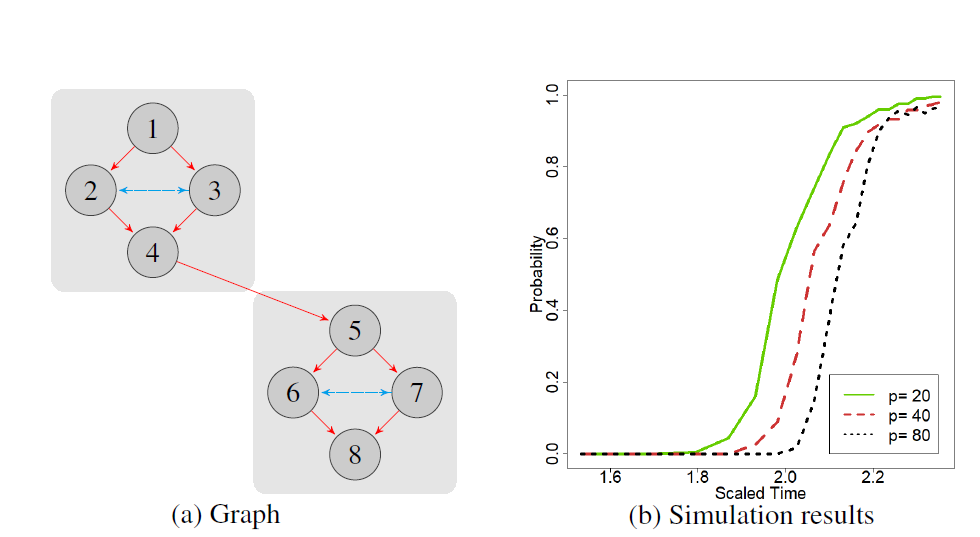
\includegraphics[height=6cm]{figure1.png}
\end{figure}



\end{frame} 







\end{document}	% Done!

